\usepackage[ngerman]{babel}
\usepackage[T1]{fontenc}
\usepackage[utf8x]{inputenc}
\usepackage{color}
\usepackage{colortbl}
\usepackage{listings}
\usepackage{longtable}
\usepackage{tikz}
\usepackage{amsthm}
\usepackage{amsmath}
\usepackage{pgfplots}
\usetikzlibrary{shapes, calc}
\usetheme[
  outer/progressbar=foot,
  outer/numbering=none
]{metropolis}

\makeatletter
\setlength{\metropolis@titleseparator@linewidth}{2pt}
\setlength{\metropolis@progressonsectionpage@linewidth}{2pt}
\setlength{\metropolis@progressinheadfoot@linewidth}{2pt}
\makeatother

\setbeamercolor{progress bar in head/foot}{fg=ffLightRed}
\setbeamercolor{title separator}{fg=ffLightRed}

\title{Freiwillige Feuerwehr Steinheim e.V.}
\subtitle{IT-Sicherheit}
\author{Dipl.-Inform. (univ.) Markus Flingelli}

\only<article>{
  \publishers{\textcopyright\ Markus Flingelli, 2019}
}

\def\datengerman{\def\today{\ifnum\day<10 0\fi\number\day.\ifnum\month<10 0\fi\number\month.\number\year}}
\date{\today}

\hypersetup{colorlinks=true, linkcolor=black, urlcolor=blue}

\setbeamercolor{frametitle}{bg=ffRed}
\newcommand{\befehl}[1]{\ttfamily #1\sf}

\DeclareMathOperator{\e}{e}
\newcommand{\iu}{{\mathrm{i}\mkern1mu}}

\AtBeginSection[]
{
  \begin{frame}<beamer>
    \frametitle{Gliederung}
    \tableofcontents[sections={\thesection}]
  \end{frame}
  \begin{frame}<handout>
    \frametitle{Gliederung}
    \tableofcontents[sections={\thesection}]
  \end{frame}
}

\renewenvironment{quotation}
  {\small\list{}{\rightmargin=0cm \leftmargin=0cm}%
   \item\relax}
  {\endlist}

\begin{document}

\only<article>{
  \thispagestyle{empty}
  \pagecolor{white}\afterpage{\nopagecolor}
  \maketitle
}

\begin{frame}[plain]
 \titlepage
\end{frame}

\only<article>{
  \section*{Vorwort}
Die Gefahren, die im Internet herrschen, werden oft unterschätzt oder nicht wahrgenommen. Das Thema IT-Sicherheit wird im privaten Umfeld oft stiefmütterlich behandelt. Unter IT-Sicher\-heit versteht man alle Planungen, Maßnahmen und Kontrollen, die dem Schutz der IT dienen.
\vspace{12pt}

Dieses Dokument soll einen kurzen Überblick über die wichtigsten Bereiche der IT-Sicherheit geben.  Des Weiteren wird aufgezeigt, welche Möglichkeiten es gibt, wie man diese erkennen und man sich davor schützen kann. Diese Ratschläge betreffen sowohl den klassischen Com\-puter- als auch den Smartphone-Nutzer.
\vspace{12pt}

Der Abschnitt zur Datenschutzgrundverordnung (DVGVO) gibt einen sehr oberflächlichen Überblick über diese und kann nicht als rechtliche Beratung gesehen werden.
\vspace{12pt}

Die Präsentation wurde ursprünglich für die Laptop-Nutzer in der FF Steinheim e.V. konzipiert. Im Rahmen der firmeninternen Ausbildung der Auszubildenden Fachininformatiker wurde sie in einer früheren Version auch in der Firma \href{https://www.blackned.de}{blackned GmbH} gehalten. Die Feuerwehrversion wurde um einige Grundlagen und aktuelle Entwicklungen ergänzt.
\vspace{24pt}

Steinheim, \today \hfill Markus Flingelli
\newpage
}

\frame{
\only<presentation>{
  \frametitle{Inhaltsverzeichnis}
}
\tableofcontents[hideallsubsections]
}
\only<article>{
  \newpage
}

\only<article>{
  \setlength\parindent{0pt}
}

\section{Sicherheitshinweise}

\subsection{Allgemein}

\begin{frame}
\only<presentation>{
	\frametitle{Allgemein}
}
\begin{itemize}
	\item Beim Verlassen des Arbeitsplatzes ist Rechner zu sperren
	\item Bei der Bearbeitung von sensiblen Daten keinen unbefugten Personen auf den Bildschirm schauen lassen
	\item Nur Software aus vertrauenswürdigen Quellen verwenden
\end{itemize}
\end{frame}

\subsection{Kennwörter}

\only<presentation>{
	\begin{frame}
\frametitle{Kennwörter}
\begin{itemize}
  \item Alle Zeichenklassen verwenden (Groß-, Kleinbuchstaben, Zahlen, Sonderzeichen)
\item Lange Passwörter (> 15 Zeichen)
\item Für jeden Dienst bzw. Webseite ein eigenes Kennwort verwenden
\item Kennwörter nicht auf Zetteln oder Post-its am Monitor notieren
\item Kennwörter können im Passwortmanager (z.B. KeePass) gespeichert werden
\end{itemize}
\end{frame}

\begin{frame}
\frametitle{Kennwörter}
\begin{itemize}
  \item Kennwörter spätestens bei Verdacht auf Missbrauch ändern
\item Voreingestellte Kennwörter ändern
\item Kennwörter nicht an Dritte weitergeben und nicht per E-Mail versenden
\item Zwei-Faktor-Authentifizierung aktivieren
\item Kennwörter regelmäßig zu ändern, wird vom BSI nicht mehr explizit gefordert
\end{itemize}
\end{frame}
}
\only<article>{
	\begin{frame}
\begin{itemize}
  \item Alle Zeichenklassen verwenden (Groß-, Kleinbuchstaben, Zahlen, Sonderzeichen)
\item Lange Passwörter (> 15 Zeichen)
\item Für jeden Dienst bzw. Webseite ein eigenes Kennwort verwenden
\item Kennwörter nicht auf Zetteln oder Post-its am Monitor notieren
\item Kennwörter können im Passwortmanager (z.B. KeePass) gespeichert werden
  \item Kennwörter spätestens bei Verdacht auf Missbrauch ändern
\item Voreingestellte Kennwörter ändern
\item Kennwörter nicht an Dritte weitergeben und nicht per E-Mail versenden
\item Zwei-Faktor-Authentifizierung aktivieren
\item Kennwörter regelmäßig zu ändern, wird vom BSI nicht mehr explizit gefordert
  \only<article>{\item BSI-Video zu Kennwörtern: \href{http://multimedia.gsb.bund.de/BSI/Video/Sicher\_im\_Internet/Passwoerter.mp4}{\url{http://multimedia.gsb.bund.de/BSI/Video/Sicher\_im\_Internet/Passwoerter.mp4}}}
\end{itemize}
\end{frame}
}

\only<presentation>{
\begin{frame}
\frametitle{Kennwörter -- BSI-Video}
BSI-Video zu Kennwörtern:\newline \href{http://multimedia.gsb.bund.de/BSI/Video/Sicher\_im\_Internet/Passwoerter.mp4}{\url{http://multimedia.gsb.bund.de/BSI/Video/Sicher\_im\_Internet/Passwoerter.mp4}}
\end{frame}
}

\only<article>{\subsubsection{Beliebteste Kennwörter 2018}}
\begin{frame}
\only<presentation>{
	\frametitle{Beliebteste Kennwörter 2018}
}
\begin{longtable}{|r|r|r|}
\hline
\rowcolor{ffLightRed} & \textcolor{white}{Passwort} & \textcolor{white}{Häufigkeit} \\
\hline
 1 & \texttt{123456}    & 8,17 ‰ \\\hline
 2 & \texttt{12345}     & 3,92 ‰ \\\hline
 3 & \texttt{123456789} & 1,91 ‰ \\\hline
 4 & \texttt{ficken}    & 1,86 ‰ \\\hline
 5 & \texttt{12345678}  & 1,40 ‰ \\\hline
 6 & \texttt{hallo123}  & 1,18 ‰ \\\hline
 7 & \texttt{hallo}     & 1,18 ‰ \\\hline
 8 & \texttt{1234}      & 1,03 ‰ \\\hline
 9 & \texttt{passwort}  & 0,98 ‰ \\\hline
10 & \texttt{master}    & 0,86 ‰ \\\hline
\end{longtable}
\scriptsize Quelle: \href{https://sec.hpi.de/ilc/statistics}{https://sec.hpi.de/ilc/statistics}
\end{frame}

\only<article>{\subsubsection{Kennwortgüte}}
\begin{frame}
\only<presentation>{
	\frametitle{Kennwortgüte}
}
\begin{longtable}{|r|r|r|r|}
\hline
\rowcolor{ffLightRed} 
\textcolor{white}{Länge} & \textcolor{white}{Ziffern (10)} & \textcolor{white}{Buchstaben (26)} & \textcolor{white}{Kombination (62)}\\
\hline
 6 &       &          &             26 s \\\hline
 7 &       &      3 s &             27 m \\\hline
 8 &       &      2 m &             28 h \\\hline
 9 &       &     42 m &             73 d \\\hline
10 &   4 s &     18 h &             12 a \\\hline
11 &  47 s &     19 d &            768 a \\\hline
12 &   8 m &      1 a &         47.639 a \\\hline
13 &  78 m &     37 a &      2.953.625 a \\\hline
14 &  13 h &    952 a &    183.124.811 a \\\hline
15 & 129 h & 24.766 a & 11.353.738.300 a \\\hline
\end{longtable}
\scriptsize Quelle: \href{https://www.1pw.de/brute-force.php}{https://www.1pw.de/brute-force.php}
\end{frame}

\subsection{Wechseldatenträger}

\begin{frame}
\only<presentation>{
	\frametitle{Wechseldatenträger}
}
\begin{itemize}
	\item Wechseldatenträger nur verwenden, wenn dessen Herkunft vertrauenswürdig ist
	\item Dateien mit vertraulichen Inhalten nur verschlüsselt ablegen (z.B. mit \href{http://www.7-zip.de/}{7-Zip} oder \href{https://www.veracrypt.fr}{VeraCrypt})
\end{itemize}
\end{frame}

\subsection{Datensicherung}

\begin{frame}
\only<presentation>{
	\frametitle{Datensicherung}
}
\begin{itemize}
	\item Regelmäßige Datensicherungen minimieren Ausfälle von Datenträgern oder Manipulationen an Datenbeständen
	\item Einspielen der Daten muss geübt werden
	\item Für Datensicherungsdatenträger gelten gleiche Sicherheitsvorgaben wie für das zu sichernde System
	\item Datensicherungen nicht im gleichen Raum oder Gebäude lagern
\end{itemize}
\end{frame}

\subsection{E-Mail}

\begin{frame}
\only<presentation>{
	\frametitle{E-Mail}
}
\begin{itemize}
	\item 3-Sekunden-Sicherheits-Check bei E-Mails
	\begin{enumerate}
		\item Ist der Absender bekannt?
		\item Ist der Betreff sinnvoll?
		\item Wird ein Anhang von diesem Absender erwartet?
	\end{enumerate}
	\item Spam-E-Mails direkt löschen
	\item Wenn möglich, E-Mails digital signieren und verschlüsseln
\end{itemize}
\end{frame}

\subsection{WLAN}

\begin{frame}
\only<presentation>{
	\frametitle{WLAN}
}
\begin{itemize}
	\item Nur sichere WLAN verwenden (WPA2)
	\item Verschlüsselung mit dem Standard WEP ist unsicher und nicht zu empfehlen
	\item Netzwerknamen (SSID) zufällig wählen (kein Rückschluss auf Betreiber oder verwendetes Gerät)
	\item Voreingestellte Kennwörter ändern
	\item WPS-PIN Verfahren deaktivieren
	\item WLAN nur bei Gebrauch einschalten
	\only<article>{\item BSI-Video zum WLAN: \href{http://multimedia.gsb.bund.de/BSI/Video/Sicher_im_Internet/WLAN.mp4}{\url{http://multimedia.gsb.bund.de/BSI/Video/Sicher\_im\_Internet/WLAN.mp4}}}
\end{itemize}
\end{frame}

\only<presentation>{
\begin{frame}
\frametitle{WLAN -- BSI-Video}
BSI-Video zum WLAN:\newline \href{http://multimedia.gsb.bund.de/BSI/Video/Sicher_im_Internet/WLAN.mp4}{\url{http://multimedia.gsb.bund.de/BSI/Video/Sicher\_im\_Internet/WLAN.mp4}}
\end{frame}
}

\subsection{Smartphones}

\only<presentation>{
	\begin{frame}
\frametitle{Smartphones}
\begin{itemize}
  \item Betriebssystem und Anwendungen (Apps) regelmäßig aktualisieren
\item Codes und Passwörter sowohl für die Entsperrung des Geräts als auch zum Öffnen von Apps sollten aktiviert und genutzt werden
\item Apps nur aus vertrauenswürdigen Quellen wie offiziellen App-Stores installieren
\item Back-up-Plan für den Fall des Verlust oder Beschädigung des Smartphones anlegen
\item Bei Verkauf oder Entsorgung Datenspeicher unwiederbringlich löschen 
\end{itemize}
\end{frame}

\begin{frame}
\frametitle{Smartphones}
\begin{itemize}
  \item Schnittstellen wie WLAN oder Bluetooth nur bei Gebrauch aktivieren
\item Vorsicht bei Nutzung offener WLAN-Hotspots (Einsatz von VPN)
\item Gerät nicht aus Augen lassen und nicht aus der Hand geben
\item Unbekannte Rufnummern nicht zurückrufen, insbesondere bei den Vorwahlen \textbf{0190} und \textbf{0180}
\item Vertrauliche Gespräche verschlüsseln
\end{itemize}
\end{frame}
}
\only<article>{
	\begin{frame}
\begin{itemize}
  \item Betriebssystem und Anwendungen (Apps) regelmäßig aktualisieren
\item Codes und Passwörter sowohl für die Entsperrung des Geräts als auch zum Öffnen von Apps sollten aktiviert und genutzt werden
\item Apps nur aus vertrauenswürdigen Quellen wie offiziellen App-Stores installieren
\item Back-up-Plan für den Fall des Verlust oder Beschädigung des Smartphones anlegen
\item Bei Verkauf oder Entsorgung Datenspeicher unwiederbringlich löschen 
  \item Schnittstellen wie WLAN oder Bluetooth nur bei Gebrauch aktivieren
\item Vorsicht bei Nutzung offener WLAN-Hotspots (Einsatz von VPN)
\item Gerät nicht aus Augen lassen und nicht aus der Hand geben
\item Unbekannte Rufnummern nicht zurückrufen, insbesondere bei den Vorwahlen \textbf{0190} und \textbf{0180}
\item Vertrauliche Gespräche verschlüsseln
\end{itemize}
\end{frame}
}

\subsection{Sicherer Umgang mit sozialen Netzwerken}

\only<presentation>{
	\begin{frame}
\frametitle{Sicherer Umgang mit sozialen Netzwerken}
\begin{itemize}
  \item Seien Sie zurückhaltend mit der Preisgabe persönlicher Informationen!
\item Erkundigen Sie sich über die Allgemeinen Geschäftsbedingungen und die Bestimmungen zum Datenschutz des genutzten sozialen Netzwerks!
\item Seien Sie wählerisch bei Kontaktanfragen -- Kriminelle \glqq sammeln\grqq\ Freunde, um Personen zu schaden!
\item Melden Sie \glqq Cyberstalker\grqq, die Sie unaufgefordert und dauerhaft über das soziale Netzwerk kontaktieren.
\end{itemize}
\end{frame}

\begin{frame}
\frametitle{Sicherer Umgang mit sozialen Netzwerken}
\begin{itemize}
  \item Verwenden Sie für jede Internetanwendung, insbesondere auch wenn Sie in verschiedenen sozialen Netzwerken angemeldet sind, ein unterschiedliches und sicheres Passwort!
\item Geben Sie keine vertraulichen Informationen über Ihren Arbeitgeber und Ihre Arbeit preis!
\item Prüfen Sie kritisch, welche Rechte Sie den Betreibern sozialer Netzwerke an den von Ihnen eingestellten Bildern, Texten und Informationen einräumen!
\item Wenn Sie \glqq zweifelhafte\grqq\ Anfragen von Bekannten erhalten, erkundigen Sie sich außerhalb sozialer Netzwerke nach der Vertrauenswürdigkeit dieser Nachricht!
\end{itemize}
\end{frame}

\begin{frame}
\frametitle{Sicherer Umgang mit sozialen Netzwerken}
\begin{itemize}
  \item Klicken Sie nicht wahllos auf Links -- Soziale Netzwerke werden verstärkt dazu genutzt, um Phishing zu betreiben!
\item Sprechen Sie mit Ihren Kindern über deren Aktivitäten in sozialen Netzwerken und klären Sie sie über die Gefahren auf!
\item Löschen eines Nutzerkontos: Erfahrungsgemäß findet sich die Möglichkeit zum Löschen eines Nutzerkontos erst nach längerem Suchen.
\end{itemize}
\end{frame}
}
\only<article>{
	\begin{frame}
\begin{itemize}
  \item Seien Sie zurückhaltend mit der Preisgabe persönlicher Informationen!
\item Erkundigen Sie sich über die Allgemeinen Geschäftsbedingungen und die Bestimmungen zum Datenschutz des genutzten sozialen Netzwerks!
\item Seien Sie wählerisch bei Kontaktanfragen -- Kriminelle \glqq sammeln\grqq\ Freunde, um Personen zu schaden!
\item Melden Sie \glqq Cyberstalker\grqq, die Sie unaufgefordert und dauerhaft über das soziale Netzwerk kontaktieren.
  \item Verwenden Sie für jede Internetanwendung, insbesondere auch wenn Sie in verschiedenen sozialen Netzwerken angemeldet sind, ein unterschiedliches und sicheres Passwort!
\item Geben Sie keine vertraulichen Informationen über Ihren Arbeitgeber und Ihre Arbeit preis!
\item Prüfen Sie kritisch, welche Rechte Sie den Betreibern sozialer Netzwerke an den von Ihnen eingestellten Bildern, Texten und Informationen einräumen!
\item Wenn Sie \glqq zweifelhafte\grqq\ Anfragen von Bekannten erhalten, erkundigen Sie sich außerhalb sozialer Netzwerke nach der Vertrauenswürdigkeit dieser Nachricht!
  \item Klicken Sie nicht wahllos auf Links -- Soziale Netzwerke werden verstärkt dazu genutzt, um Phishing zu betreiben!
\item Sprechen Sie mit Ihren Kindern über deren Aktivitäten in sozialen Netzwerken und klären Sie sie über die Gefahren auf!
\item Löschen eines Nutzerkontos: Erfahrungsgemäß findet sich die Möglichkeit zum Löschen eines Nutzerkontos erst nach längerem Suchen.
\end{itemize}
\end{frame}
}

\section{DSGVO}

\subsection{Allgemeines}
\begin{frame}
\only<presentation>{
	\frametitle{Allgemeines}
}
\begin{itemize}
	\item Nur notwendige Daten speichern (Datensparsamkeit)
	\item Bei Verarbeitung personenbezogener Daten muss angemessene Sicherheit gewährleistet werden
	\item Gesetzliche Speicherfristen sind zu beachten
	\item Auskunftsrecht des Betroffenen
	\item Informationsrecht bei Erhebung von Nutzerdaten
	\item Sicherheit der Verarbeitung
	\item IT-Sicherheitsvorgaben befolgen
\end{itemize}
\end{frame}

\subsection{Technische und organisatorische Maßnahmen}
\begin{frame}
\only<presentation>{
	\frametitle{Technische und organisatorische Maßnahmen}
}
\begin{itemize}
	\item Zustimmung zum Erfassen muss gegeben sein
	\item Einlegen von Widerspruch zur Datenerfassung muss gewährleistet sein
	\item Einsicht in erhobenen Daten muss möglich sein
	\item Verwendungszweck der Daten muss erfragt werden können
	\item Daten müssen sich berichtigen lassen können
	\item Daten müssen unter Umständen gesperrt werden können
\end{itemize}
\end{frame}

\section{Spam}

\subsection{Grundbegriffe}

\only<article>{\subsubsection{Exkurs}}

\begin{frame}
\only<presentation>{
	\frametitle{Exkurs: Ursprung des Begriffs}
}
\begin{itemize}
	\item SPAM war ursprünglich ein Markenname für Dosenfleisch, der bereits 1936 entstanden ist, aus \textit{\textbf{SP}iced h\textbf{AM}} (gewürzter Schinken)
	\item SPAM in der IT geht vermutlich auf einen am 15.12.1970 erstausgestrahlten Sketch von Monty Python zurück
	\item Sketch spielt in Café, in dem fast jedes Gericht aus SPAM besteht
	\item In dem knapp zweiminütigem Sketch wird 132-mal das Wort SPAM verwendet
	\item Video: \href{https://www.dailymotion.com/video/x2hwqlw}{SPAM-Sketch} (Englisch)
\end{itemize}
\end{frame}

\only<article>{\subsubsection{Definitionen}}
\begin{frame}
\only<presentation>{
	\frametitle{Grundbegriffe}
}
Spam bezeichnet den Massenversand nichtangeforderter Werbe-E-Mails und kann in folgende Bereiche unterteilt werden:
\begin{description}
	\item[Phising] Abfangen vertraulicher Daten wie Passwörter, Zugangsdaten oder Kreditkartennummern
	\item[Hoax] Falschmeldungen, die vergleichbar mit Zeitungsenten, im Internet kursieren
	\item[Scam] Scam-Mails enthalten Gewinnversprechen bzw. das Versprechen, schnell und mit einfachen Mitteln reich zu werden
\end{description}
\end{frame}

\only<presentation>{
	\begin{frame}
\frametitle{Erkennen von Phising-E-Mails}
\begin{itemize}
  \item Die Absenderadressen sind zumeist gefälscht.
\item Die Anrede ist unpersönlich gehalten.
\item Dringender Handlungsbedarf wird signalisiert.
\item Drohungen kommen zum Einsatz.
\item Vertrauliche Daten (wie beispielsweise PINs und TANs) werden abgefragt, etwa in einem Formular innerhalb der E-Mail.
\item Die Mails enthalten Links oder Formulare, die vom Empfänger verfolgt beziehungsweise geöffnet werden sollen.
\end{itemize}
\end{frame}

\begin{frame}
\frametitle{Erkennen von Phising-E-Mails}
\begin{itemize}
  \item Die Nachrichten sind manchmal (aber nicht immer!) in schlechtem Deutsch verfasst. Die Gründe dafür: Sie werden manchmal von Computerprogrammen aus anderen Sprachen automatisch übersetzt.
\item Die E-Mails enthalten kyrillische Buchstaben oder falsch aufgelöste bzw. fehlende Umlaute (z.B. nur \glqq a\grqq\ statt \glqq ä\grqq\ beziehungsweise \glqq ae\grqq).
\end{itemize}
\end{frame}
}
\only<article>{
	\subsection{Erkennen von Phising-E-Mails}
	\begin{frame}
\begin{itemize}
  \item Die Absenderadressen sind zumeist gefälscht.
\item Die Anrede ist unpersönlich gehalten.
\item Dringender Handlungsbedarf wird signalisiert.
\item Drohungen kommen zum Einsatz.
\item Vertrauliche Daten (wie beispielsweise PINs und TANs) werden abgefragt, etwa in einem Formular innerhalb der E-Mail.
\item Die Mails enthalten Links oder Formulare, die vom Empfänger verfolgt beziehungsweise geöffnet werden sollen.
  \item Die Nachrichten sind manchmal (aber nicht immer!) in schlechtem Deutsch verfasst. Die Gründe dafür: Sie werden manchmal von Computerprogrammen aus anderen Sprachen automatisch übersetzt.
\item Die E-Mails enthalten kyrillische Buchstaben oder falsch aufgelöste bzw. fehlende Umlaute (z.B. nur \glqq a\grqq\ statt \glqq ä\grqq\ beziehungsweise \glqq ae\grqq).
  \item BSI-Video zu Phising: \href{http://multimedia.gsb.bund.de/BSI/Video/Sicher\_im\_Internet/Phishing.mp4}{\url{http://multimedia.gsb.bund.de/BSI/Video/Sicher\_im\_Internet/Phishing.mp4}}
\end{itemize}
\end{frame}
}

\only<presentation>{
\begin{frame}
\frametitle{Erkennen von Phising-E-Mails -- BSI-Video}
BSI-Video zu Phising:\newline \href{http://multimedia.gsb.bund.de/BSI/Video/Sicher\_im\_Internet/Phishing.mp4}{\url{http://multimedia.gsb.bund.de/BSI/Video/Sicher\_im\_Internet/Phishing.mp4}}
\end{frame}
}


\subsection{Beispiele}

\only<article>{\subsubsection{Falsche Telekom-Rechnung}}

\begin{frame}
\only<presentation>{
  \frametitle{Falsche Telekom-Rechnung}
}
\only<article>{
  \begin{enumerate}
  \item[1] Absenderadresse entspricht nicht der Telekom
  \item[2] Seriöse Anbieter verschicken keine Rechnungen als Word-Dokumente (Gefahr von Viren)
  \item[3] Keine persönliche Anrede
  \item[4] Grammatikalischer Fehler
  \end{enumerate}
}
\begin{figure}[ht]
	\centering
	\only<presentation>{
		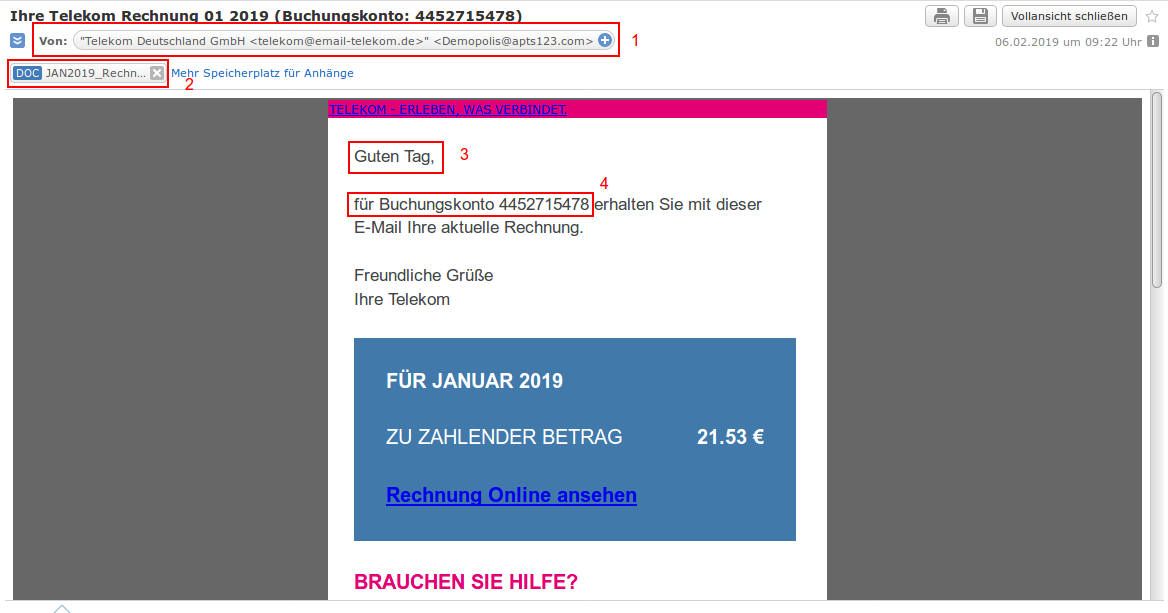
\includegraphics[width=.95\textwidth]{fake_telekom_rechnung_kommentar.png}
	}
	\only<article>{
	  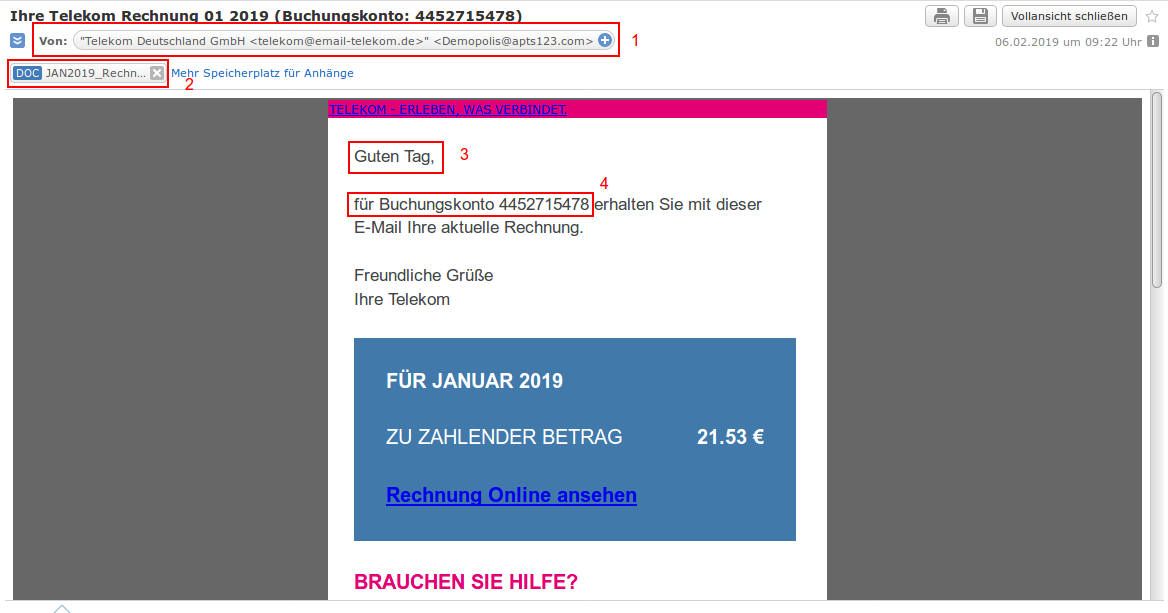
\includegraphics[width=.80\textwidth]{fake_telekom_rechnung_kommentar.png}
	}
\end{figure}
\end{frame}

\only<article>{\subsubsection{Falscher Microsoft-Servicevertrag}}

\begin{frame}
\only<presentation>{
  \frametitle{Falscher Microsoft-Servicevertrag}
}
\only<article>{
  \begin{enumerate}
  \item[1] Absenderadresse gehört nicht zu Microsoft
  \item[2] Keine persönliche Begrüßung
  \end{enumerate}
}
\begin{figure}[ht]
	\centering
	\only<presentation>{
		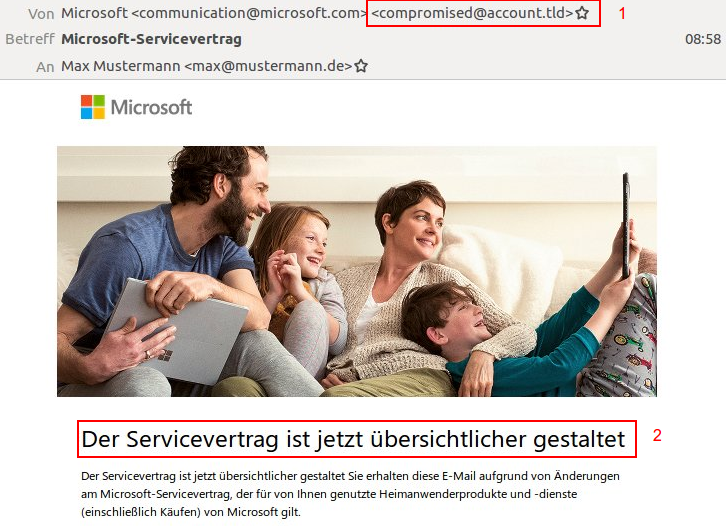
\includegraphics[width=.9\textwidth]{fake_microsoft_email.png}
	}
	\only<article>{
	  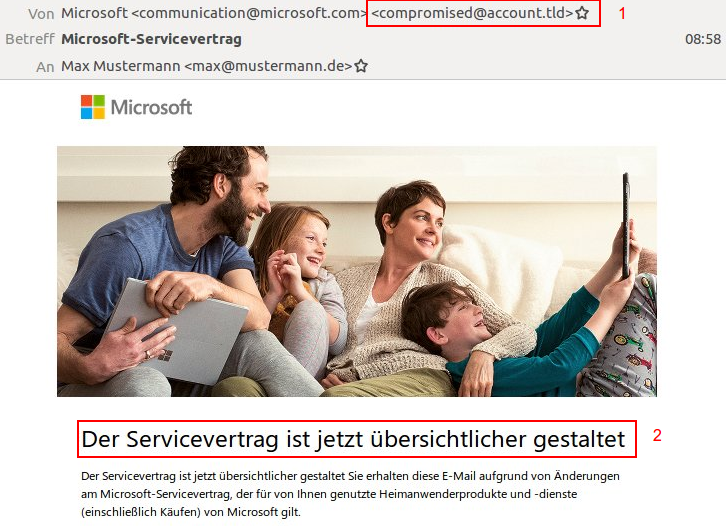
\includegraphics[width=.50\textwidth]{fake_microsoft_email.png}
	}
\end{figure}
\end{frame}

\only<article>{\subsubsection{Hoax}}

\begin{frame}
\only<presentation>{
	\frametitle{Hoax}
}
\begin{quotation}
Hi Leute,

ich wende mich an Euch, weil ich ziemlich verzweifelt bin. Ich hoffe, Ihr könnt mir und meiner Freundin helfen, und lest diesen Brief! Das Problem ist, dass meine Freundin an Leukämie erkrankt ist. Es hat sich herausgestellt, dass Sie nur noch wenige Wochen zu Leben hat. Aus diesem Grund seit Ihr meine letzte Chance Ihr zu helfen. 
[...]

Ich danke Euch für Eure Hilfe!!!

Gruß Toshiba65@aol.com
\end{quotation}
\end{frame}

\only<article>{\subsubsection{Scam}}

\begin{frame}
\only<presentation>{
	\frametitle{Scam}
}
\begin{quotation}
Sehr geehrter Herr,

Ich bin an Ihrer Geschäftspartnerschaft interessiert. Das Angebot, mit dem ich an Sie herantrete, ist für beide Seiten von Vorteil und sein Erfolg gründet sich auf gegenseitiges Vertrauen und gegenseitige Zusammenarbeit und einen hohen Grad an Vertraulichkeit, was diese Transaktion betrifft. Ich repräsentiere den Vorstand der Vertrags- und Aufsichtsabteilung des Zambianischen Ministeriums für Bergbau und Ressourcen. Ich bitte Sie um Ihre Hilfe, um den Transfer der Summe von etwa USD 30.500.000,00 (DREISSIG MILLIONEN FÜNFHUNDERT TAUSEND DOLLAR) auf Ihr Bankkonto zu ermöglichen.
\end{quotation}
\end{frame}

\section{Sicherheitsirrtümer}

\subsection{Internet-Sicherheit}

\only<presentation>{
	\begin{frame}
\frametitle{Internet-Sicherheit}
\begin{itemize}
  \item Sicherheitsvorkehrungen sind unnötig, die Hacker knacken doch sowieso alles.
\item Meine PC-Firewall schützt mich vor allen Angriffen aus dem Internet.
\item Wenn ich ein aktuelles Virenschutzprogramm habe, muss ich Updates für andere Software nicht sofort installieren.
\item Ein einziges langes Buchstaben- und Zeichen-Passwort reicht für meine Online-Dienste vollkommen aus.

\end{itemize}
\end{frame}

\begin{frame}
\frametitle{Internet-Sicherheit}
\begin{itemize}
  \item Ich surfe nur auf vertrauenswürdigen Seiten, darum muss ich mich nicht vor Cyber-Angriffen schützen.
\item Wenn der eigene Rechner infiziert ist, merkt man das.
\item Ich surfe nicht auf Pornoseiten, deshalb kann ich mir nichts einfangen.
\item Sehe ich das Schloss im Browser, ist alles in Ordnung.
\end{itemize}
\end{frame}
}
\only<article>{
	\begin{frame}
\begin{itemize}
  \item Sicherheitsvorkehrungen sind unnötig, die Hacker knacken doch sowieso alles.
\item Meine PC-Firewall schützt mich vor allen Angriffen aus dem Internet.
\item Wenn ich ein aktuelles Virenschutzprogramm habe, muss ich Updates für andere Software nicht sofort installieren.
\item Ein einziges langes Buchstaben- und Zeichen-Passwort reicht für meine Online-Dienste vollkommen aus.

  \item Ich surfe nur auf vertrauenswürdigen Seiten, darum muss ich mich nicht vor Cyber-Angriffen schützen.
\item Wenn der eigene Rechner infiziert ist, merkt man das.
\item Ich surfe nicht auf Pornoseiten, deshalb kann ich mir nichts einfangen.
\item Sehe ich das Schloss im Browser, ist alles in Ordnung.
\end{itemize}
\end{frame}
}


\subsection{Mobile Sicherheit}

\begin{frame}
\only<presentation>{
	\frametitle{Mobile Sicherheit}
}
\begin{itemize}
	\item Meine Daten sind in der Cloud sicher vor Fremdzugriff geschützt.
	\item Das Surfen in öffentlichen WLANs spart nicht nur Kosten, sondern ist auch sicher.
	\item Wenn ich mir ein neues Smartphone kaufe, habe ich automatisch ein sicheres Gerät.
	\item Ich habe natürlich automatische Updates und Aktualisierungen des Betriebssystems und von Apps aktiviert, daher muss ich mich um Schwachstellen nicht kümmern.
\end{itemize}
\end{frame}

\subsection{Computer-Sicherheit}

\only<presentation>{
	\begin{frame}
\frametitle{Computer-Sicherheit}
\begin{itemize}
  \item Wenn ich einen Virus oder ein anderes Schadprogramm auf dem Computer habe, macht sich dieser auch bemerkbar.
\item Ich habe nichts zu verbergen und keine wichtigen Daten, also bin ich doch kein Ziel für Cyber-Kriminelle und muss mich deshalb nicht schützen.
\item Meine Daten sind doch in der Cloud, darum brauche ich kein Back-up.

\end{itemize}
\end{frame}

\begin{frame}
\frametitle{Computer-Sicherheit}
\begin{itemize}
  \item Wenn ich alle Daten von meinem Gerät lösche und anschließend den Papierkorb leere, sind die Daten ein für alle mal weg.
\item Wenn ich ein gutes Kennwort habe, dann kann keiner meine E-Mails lesen.
\item Geheime Sicherheitsverfahren sind immer sicherer als öffentlich bekannte Verfahren.
\end{itemize}
\end{frame}
}
\only<article>{
	\begin{frame}
\begin{itemize}
  \item Wenn ich einen Virus oder ein anderes Schadprogramm auf dem Computer habe, macht sich dieser auch bemerkbar.
\item Ich habe nichts zu verbergen und keine wichtigen Daten, also bin ich doch kein Ziel für Cyber-Kriminelle und muss mich deshalb nicht schützen.
\item Meine Daten sind doch in der Cloud, darum brauche ich kein Back-up.

  \item Wenn ich alle Daten von meinem Gerät lösche und anschließend den Papierkorb leere, sind die Daten ein für alle mal weg.
\item Wenn ich ein gutes Kennwort habe, dann kann keiner meine E-Mails lesen.
\item Geheime Sicherheitsverfahren sind immer sicherer als öffentlich bekannte Verfahren.
\end{itemize}
\end{frame}
}

\subsection{E-Mail}

\begin{frame}
\only<presentation>{
	\frametitle{E-Mail}
}
\begin{itemize}
	\item Wenn ich eine E-Mail nur anschaue, aber keinen Anhang öffne, kann nichts passieren.
	\item Das Antworten auf Spam-Mails birgt keine Gefahr, man kann auch den Links zum Löschen aus dem Verteiler folgen.
	\item Eine E-Mail kommt immer von der Adresse, die im Absenderfeld steht.
	\item Phishing-Mails sind leicht zu erkennen.
	\item Ich öffne nur Mails von Freunden und Bekannten, deshalb kann mir nichts passieren.
\end{itemize}
\end{frame}

\subsection{Computer-Sicherheit}

\only<presentation>{
	\begin{frame}
\frametitle{Computer-Sicherheit}
\begin{itemize}
  \item Wenn ich einen Virus oder ein anderes Schadprogramm auf dem Computer habe, macht sich dieser auch bemerkbar.
\item Ich habe nichts zu verbergen und keine wichtigen Daten, also bin ich doch kein Ziel für Cyber-Kriminelle und muss mich deshalb nicht schützen.
\item Meine Daten sind doch in der Cloud, darum brauche ich kein Back-up.

\end{itemize}
\end{frame}

\begin{frame}
\frametitle{Computer-Sicherheit}
\begin{itemize}
  \item Wenn ich alle Daten von meinem Gerät lösche und anschließend den Papierkorb leere, sind die Daten ein für alle mal weg.
\item Wenn ich ein gutes Kennwort habe, dann kann keiner meine E-Mails lesen.
\item Geheime Sicherheitsverfahren sind immer sicherer als öffentlich bekannte Verfahren.
\end{itemize}
\end{frame}
}
\only<article>{
	\begin{frame}
\begin{itemize}
  \item Wenn ich einen Virus oder ein anderes Schadprogramm auf dem Computer habe, macht sich dieser auch bemerkbar.
\item Ich habe nichts zu verbergen und keine wichtigen Daten, also bin ich doch kein Ziel für Cyber-Kriminelle und muss mich deshalb nicht schützen.
\item Meine Daten sind doch in der Cloud, darum brauche ich kein Back-up.

  \item Wenn ich alle Daten von meinem Gerät lösche und anschließend den Papierkorb leere, sind die Daten ein für alle mal weg.
\item Wenn ich ein gutes Kennwort habe, dann kann keiner meine E-Mails lesen.
\item Geheime Sicherheitsverfahren sind immer sicherer als öffentlich bekannte Verfahren.
\end{itemize}
\end{frame}
}

\section{Mehrfachnutzung Computer}

\only<presentation>{
	\begin{frame}
\frametitle{Computer-Mehrfachnutzung}
\begin{itemize}
  \item Nicht mit Administratorenrechten arbeiten
\item Unterschiedliche Benutzerkonten einrichten
\item Immer aktuelle Software einsetzen
\item Nutzungsberechtigungen einschränken
\item Nutzungsmöglichkeiten für Kinder einschränken

\end{itemize}
\end{frame}

\begin{frame}
\frametitle{Computer-Mehrfachnutzung}
\begin{itemize}
  \item Sensible Daten auf separaten Geräten bearbeiten
\item Vorsichtig mit Passwörtern umgehen
\item Verlauf löschen und wenn möglich, Inkognito-Modus verwenden
\item Daten regelmäßig sichern
\end{itemize}
\end{frame}
}
\only<article>{
	\begin{frame}
\begin{itemize}
  \item Nicht mit Administratorenrechten arbeiten
\item Unterschiedliche Benutzerkonten einrichten
\item Immer aktuelle Software einsetzen
\item Nutzungsberechtigungen einschränken
\item Nutzungsmöglichkeiten für Kinder einschränken

  \item Sensible Daten auf separaten Geräten bearbeiten
\item Vorsichtig mit Passwörtern umgehen
\item Verlauf löschen und wenn möglich, Inkognito-Modus verwenden
\item Daten regelmäßig sichern
\end{itemize}
\end{frame}
}

\section{Hacking}

\begin{frame}
\only<presentation>{
  \frametitle{Abgreifen Zugangsdaten}
}
\begin{itemize}
	\item Anmeldung auf der Website \href{http://steinheim.ffw-mm.de/}{http://steinheim.ffw-mm.de/}
	\item Verwendeter Nutzername: \textbf{flingo}
	\item Verwendetes Kennwort: \textbf{MeinKennwortVerateichnicht}
\end{itemize}
\end{frame}

\begin{frame}
\only<presentation>{
  \frametitle{Abgreifen Zugangsdaten}
}
\only<article>{
	\newpage
	Das Abgreifen der Zugangsdaten ist möglich, da die Verbindung zur Webseite nicht abgesichert ist.
}
\begin{figure}[ht]
	\centering
	\only<presentation>{
		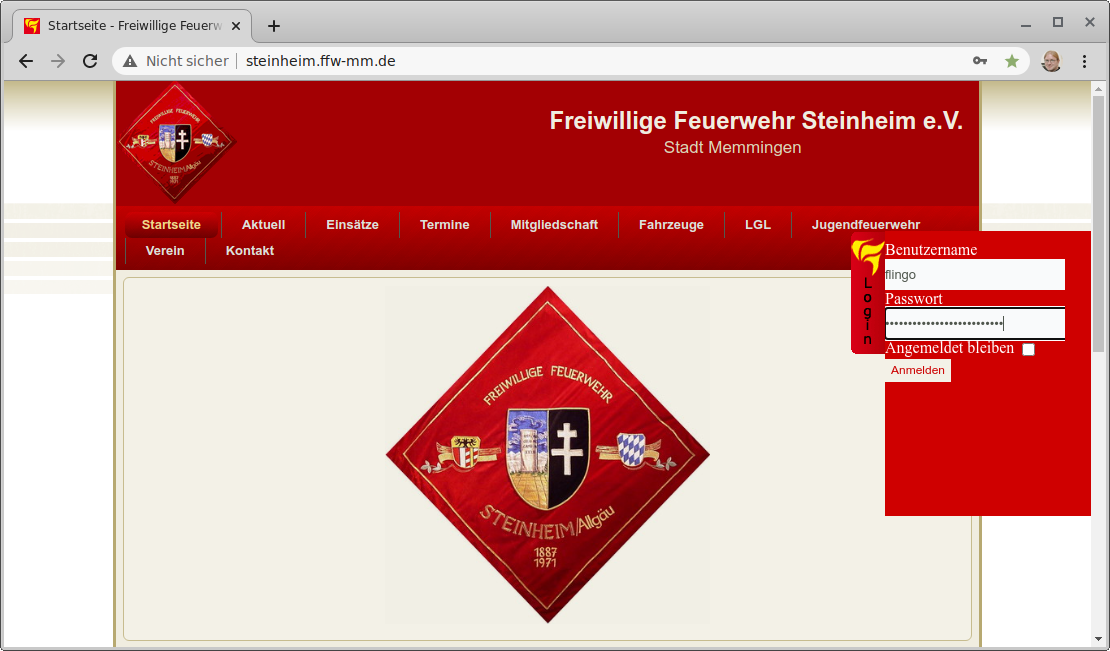
\includegraphics[width=.95\textwidth]{webseite_steinheim.png}
	}
	\only<article>{
	  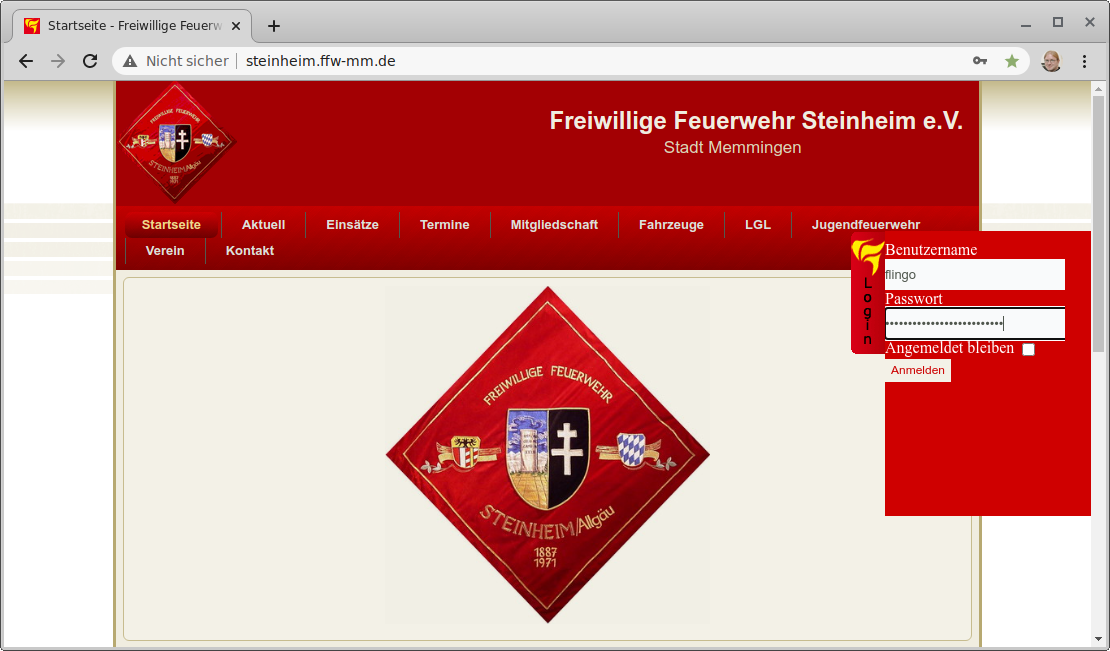
\includegraphics[width=.80\textwidth]{webseite_steinheim.png}
	}
\end{figure}
\end{frame}

\begin{frame}
\only<presentation>{
  \frametitle{Abgreifen Zugangsdaten}
}
\only<article>{
	Das Abgreifen der Zugangsdaten kann beispielsweise über Wireshark erfolgen. Wireshark ist eine Anwendung, die frei im Internet verfügbar ist.
}
\begin{figure}[ht]
	\centering
	\only<presentation>{
		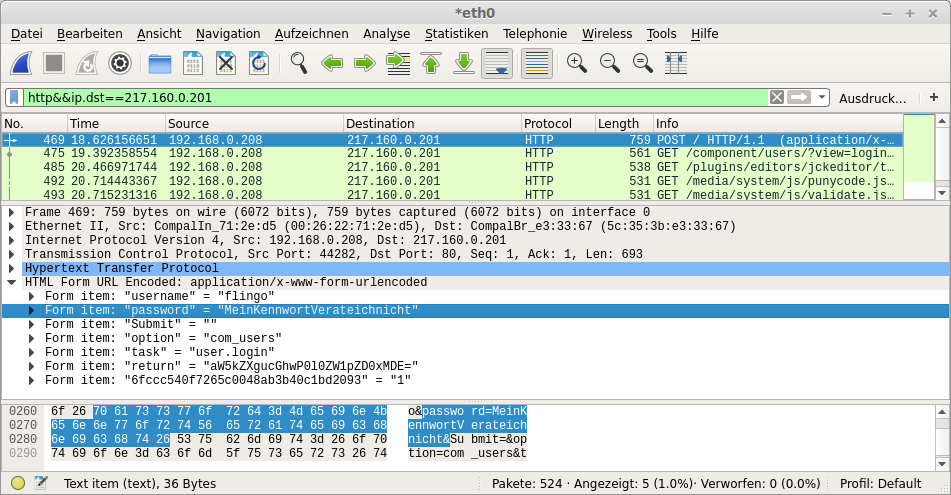
\includegraphics[width=\textwidth]{http_kennwort.png}
	}
	\only<article>{
	  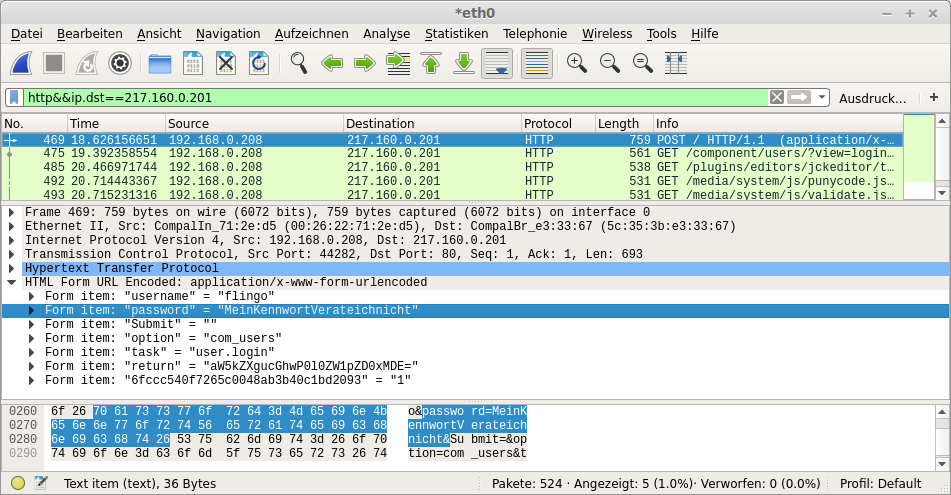
\includegraphics[width=.80\textwidth]{http_kennwort.png}
	}
\end{figure}
\end{frame}

\begin{frame}
\only<presentation>{
  \frametitle{Abgreifen Zugangsdaten}
}
\only<article>{
	Das Programm nslookup erlaubt das Auflösen von Namen zu Internetadressen. Dieses Programm ist auf allen gängigen Betriebsystemen wie Windows, Linux und MacOS verfügbar.
	\newpage
}
\begin{figure}[ht]
	\centering
	\only<presentation>{
		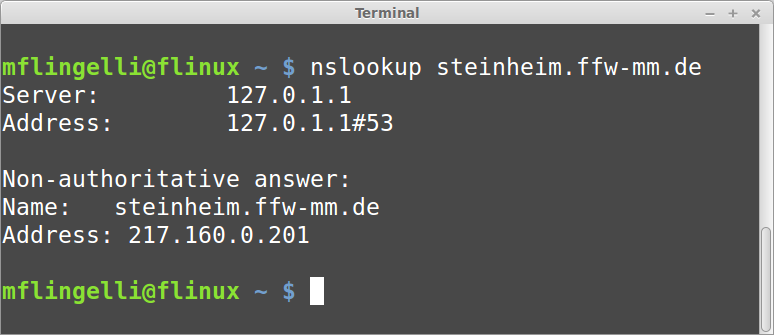
\includegraphics[width=\textwidth]{nslookup_steinheim.png}
	}
	\only<article>{
	  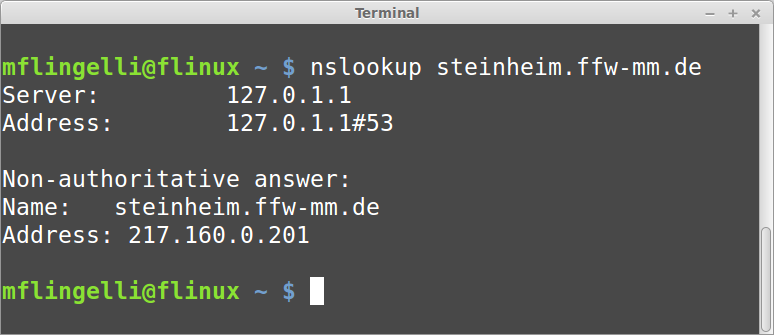
\includegraphics[width=.80\textwidth]{nslookup_steinheim.png}
	}
\end{figure}
\end{frame}

\section{Weiterführende Informationen}

\begin{frame}
\only<presentation>{
	\frametitle{Weiterführende Informationen}
}
\begin{itemize}
	\item BSI für Bürger -- Ins Internet mit Sicherheit:  \href{https://www.bsi-fuer-buerger.de}{https://www.bsi-fuer-buerger.de}
	\item Datenschutzgrundsätze in Deutschland: \href{https://www.datenschutz.org/datenschutzgrundsaetze/}{https://www.datenschutz.org/datenschutzgrundsaetze/}
	\item Fraunhofer-Institut für sichere Informationstechnologie: \href{https://www.sit.fraunhofer.de/fileadmin/dokumente/sonstiges/Security-Mythen.pdf}{Security Mythen}
	\item Landesfeuerwehrverband Bayern: \href{https://www.lfv-bayern.de/aktuelles/datenschutz-im-verein-und-die-neue-datenschutz-grundverordnung/}{https://www.lfv-bayern.de/aktuelles/datenschutz-im-verein-und-die-neue-datenschutz-grundverordnung/}
\end{itemize}
\end{frame}

\only<presentation>{
\begin{frame}
	\frametitle{Fragen?}
	\begin{figure}[ht]
		\centering
		
\includegraphics[height=.75\textheight]{homer_pythagoras.png}
	\end{figure}
	\scriptsize{Quelle: \href{https://vividkaret.files.wordpress.com/2014/10/homer.png}{\url{https://vividkaret.files.wordpress.com/2014/10/homer.png}}}
\end{frame}
}

\makeatletter
\only<article>{
  \ifthispageodd{
  }{
    \newpage
    \null
  }
  \clearpage
  \newpage
  \thispagestyle{empty}
  \pagecolor{Titelhintergrundfarbe}\afterpage{\nopagecolor}
  \vspace*{175mm}
  \linespread{1.25}
  \begin{flushright}
    \large\textcolor{Titelfarbe}{Ersteller: \@author}\\
    \large\textcolor{Titelfarbe}{Letzte \"Anderung: \@date}\\
    \large\textcolor{Titelfarbe}{\@publishers}
  \end{flushright}
  \linespread{1}
}
\makeatother

\end{document}